\chapter{Background}\label{ch:background}

The following sections provide an overview of the main concepts and technologies that are relevant to the work presented in this thesis: \acrshort{dt}s, smart homes, and automations for smart devices.

\section{Digital Twins}

A \acrfull{dt} is a computer-based model that simulates, mirrors, or ``twins'' the life of a physical entity, such as an object, a process, a human, or a human-related feature \parencite{barricelliMultiModalApproachCreating2022}.

A \acrshort{dt} is more than a passive copy; it is an intelligent and adaptive system that acts as the living counterpart to its physical twin \parencite{grievesDigitalTwinManufacturing2014,kritzingerDigitalTwinManufacturing2018}. It continuously  monitors, analyzes, and optimizes the real-world entity throughout its lifecycle \parencite{negriReviewRolesDigital2017}. This allows for proactive maintenance and prevention of issues like defects and failures, as well as experimentation and optimization through simulations of new scenarios. The twinning process is enabled by the dynamic interplay between the \acrshort{dt}, its physical twin, and the surrounding environment---a continuous loop of interaction, communication, and improvement.

The \acrshort{dt} keeps track of its physical twin and environment through real-time data streams and extensive data storage capabilities. Descriptive data exchanges, facilitated by big data infrastructure, ensure consistent alignment with the physical system. Advanced algorithms, including data fusion, big data analytics, and \acrshort{ai}-based descriptive methods, are used to extract valuable insights from this rich data source. The modular and highly parameterized architecture of the \acrshort{dt} allows for quick reconfiguration, enabling it to evolve along with its physical twin. This synchronization ensures the \acrshort{dt} always reflects the properties and changes happening in the real world.

Leveraging its \acrshort{ai} capabilities, the \acrshort{dt} goes beyond mere emulation by discovering hidden patterns, unknown correlations, and comprehensive system descriptions. This holistic understanding of the physical system, along with the ability to record, control, and monitor its state, enables techniques for failure prediction, solution simulation, and even self-healing mechanisms. This powerful combination enables a predictive maintenance approach, where proactive actions prevent failures and optimize performance through simulated testing and solution selection.

Despite their inherent intelligence, \acrshort{dt}s are not meant to operate in total autonomy.\@ \acrshort{ai}-based applications and \acrshort{dt}s often need significant human input, especially when testing new features and modifications on physical assets, or when the systems are used to provide critical outputs like medical diagnoses and treatment recommendations \parencite{barricelliSurveyDigitalTwin2019}.

\subsection{Historical Notes}

The term \textit{digital twin} was coined by Michael Grieves in 2002, in the context of \acrfull{plm} \parencite{grievesDigitalTwinManufacturing2014,grievesDigitalTwinMitigating2017}. He defined a \acrshort{dt} as a virtual representation of a physical object, connected by a bidirectional flow of data and information. Figure~\ref{fig:grieves_digital_twin} illustrates his \acrshort{dt} model, which consists of three main components:
\begin{enumerate}
    \item A physical space, where the real object exists and operates;
    \item A virtual space, where the digital object is created and simulated;
    \item A connection to transfer data from the physical to the virtual space, and information from the virtual space to the physical space. This is essential for achieving alignment and synchronization between the virtual and physical systems.
\end{enumerate}

\begin{figure}
    \centering
    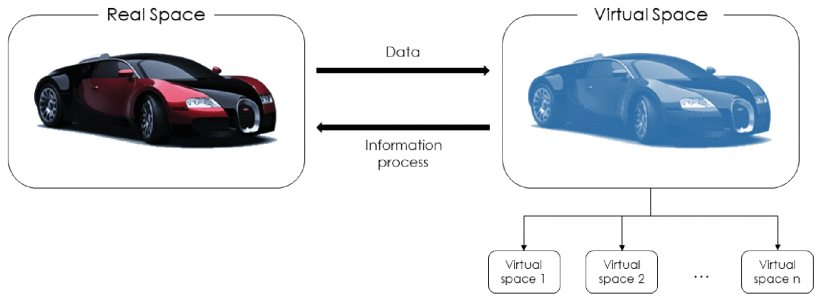
\includegraphics[width=0.8\textwidth]{images/digital_twins/dt_model_grieves.png}
    \caption[Grieves' \acrshort{dt} model]{Grieves' \acrshort{dt} model. From \textcite{barricelliSurveyDigitalTwin2019}, \textit{Research Background} section, CC-BY 4.0 license}%
    \label{fig:grieves_digital_twin}
\end{figure}

Building on Grieves' idea, \textcite{framlingProductAgentsHandling2003} proposed ``an agent-based architecture where each product item has a corresponding virtual counterpart or agent associated with it''. They envisioned that these agents would leverage the ubiquitous connectivity of the Internet to maintain synchronization with their physical counterparts, and also offer services for them \parencite{framlingProductAgentsHandling2003}. Their motivation was that a robust \acrshort{plm} system should have a reliable and up-to-date view of the product's status and information, throughout its entire lifecycle.

\acrshort{dt}s garnered much interest in the aerospace and defense industries~\parencite{negriReviewRolesDigital2017}. NASA explored \acrshort{dt}s as a way to save costs and resources for its space missions. Their study resulted in a roadmap that validated the value of \acrshort{dt}s in enhancing performance in the aviation domain. They described the DT as ``an integrated multi-physics, multi-scale, probabilistic simulation of a vehicle or system that uses the best available physical models, sensor updates, fleet history, etc., to mirror the life of its flying twin. The \acrshort{dt} is ultra-realistic and may consider one or more important and interdependent vehicle systems, including propulsion/energy storage, avionics, life support, vehicle structure, thermal management/TPS, etc.\''~\parencite{shaftoModelingSimulationInformation2010}. The U.S. Air Force also created the \acrfull{adt}, a computational model of individual aircrafts, which aimed to improve the way U.S. Air Force aircrafts were maintained over their entire lifecycle by generating personalized structural management plans~\parencite{tuegelAirframeDigitalTwin2012,gockelChallengesStructuralLife2012}.

Moreover, \acrshort{dt}s are also a key element of Industry 4.0~\parencite{brettelHowVirtualizationDecentralization2014,hermannDesignPrinciplesIndustrie2016,vachalekDigitalTwinIndustrial2017,negriReviewRolesDigital2017}, where they are applied to monitor and optimize the performance of manufacturing systems, and to facilitate the development of new products and services. The \acrshort{dt} is a catalyst for the digital transformation of the manufacturing industry, and it is a vital component of the smart factory \parencite{mabkhotRequirementsSmartFactory2018}.

\subsection{Design of Digital Twins}\label{sec:dt_design}

\acrshort{dt}s can have two different lifecycles, depending on whether the objects they represent are already existing or not~\parencite{barricelliSurveyDigitalTwin2019}. The first lifecycle applies to objects that are still in the design stage, and involves creating both the object and its \acrshort{dt} simultaneously. The second lifecycle applies to objects that already exist, but do not have a \acrshort{dt} yet. In this case, the design process aims to equip the objects with connectivity features to enable their \acrshort{dt} creation. Both lifecycles follow the same sequence: a \textit{design} phase, a \textit{development} phase, an \textit{operational} phase, and a \textit{dismissal} phase.

\begin{figure}
    \centering
    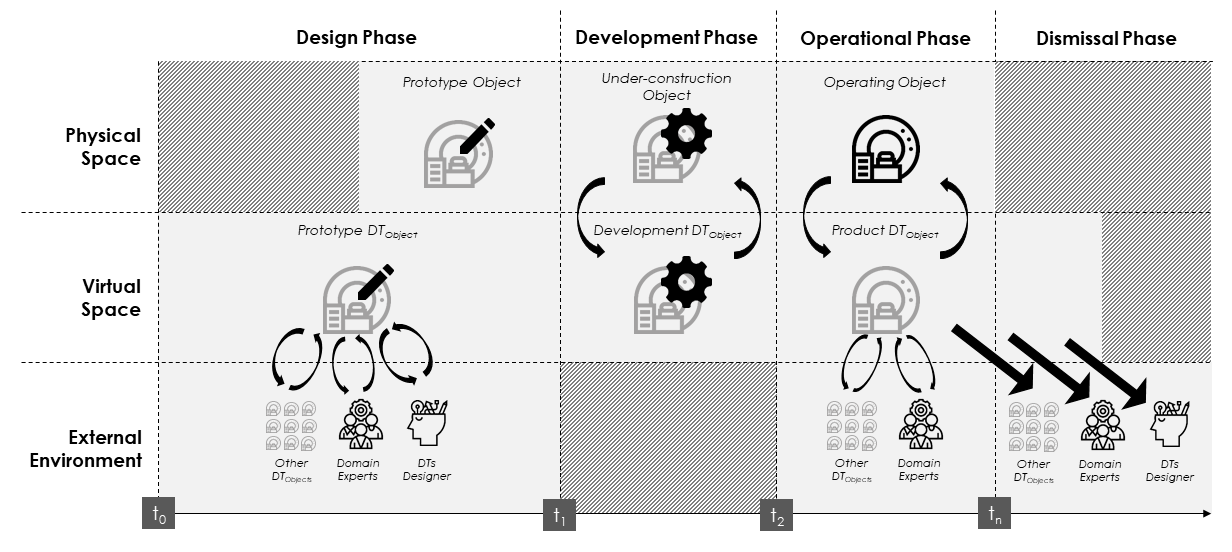
\includegraphics[width=0.9\textwidth]{images/digital_twins/dt_lifecycle_1.png}
    \caption[Lifecycle of a \acrshort{ct} scanner and its \acrshort{dt}, starting from the development of the \acrshort{dt}]{Lifecycle of a \acrshort{ct} scanner and its \acrshort{dt}, starting from the development of the \acrshort{dt}. From \textcite{barricelliSurveyDigitalTwin2019}, \textit{Design Implications} section, CC-BY 4.0 license}%
    \label{fig:dt_lifecycle_1}
\end{figure}

To illustrate these two lifecycles, a \acrfull{ct} scanner is used as an example. The first lifecycle is shown in Figure~\ref{fig:dt_lifecycle_1}. The \acrshort{dt} is created before the physical object as a prototype \(DT_{object}\), which assists the designers in the design phase of the prototype object. The prototype \(DT_{object}\) serves as a virtual model of the real prototype, enabling the designers to simulate, test, modify, and validate their design choices using data from the prototype \(DT_{object}\) and other sources. When the prototype \(DT_{object}\) is finalized, the design phase shifts to the prototype object, where the prototype \(DT_{object}\) may be revised to address any technical issues. In the development phase, the prototype \(DT_{object}\) becomes a development \(DT_{object}\), which interacts with the production machines to monitor and optimize the assembly/construction of the object, i.e., its physical twin. When the object is built, the development \(DT_{object}\) becomes a product \(DT_{object}\), and the operational phase begins. The product \(DT_{object}\) corresponds to the object and tracks and mirrors the \acrshort{dt} scanner while it is in use. The product \(DT_{object}\) also learns and adapts to the object during its operation. When the object is no longer used, the dismissal phase starts, first for the object and then for the \(DT_{object}\). The historical data of the product \(DT_{object}\) are backed up and shared with other \acrshort{dt}s and domain experts so that they can use the information to improve the production of future devices.

\begin{figure}
    \centering
    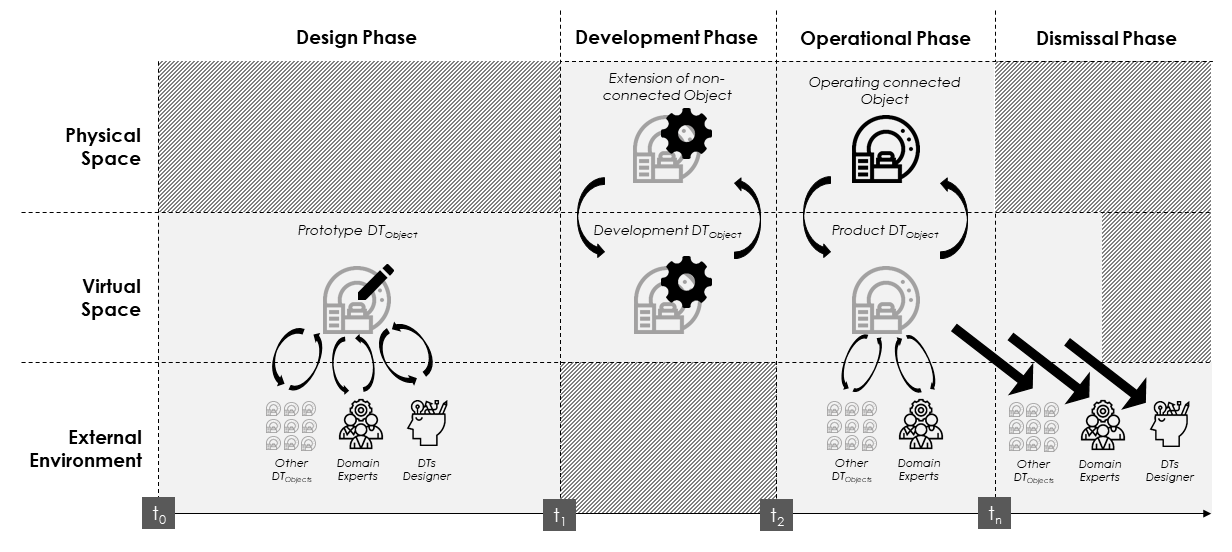
\includegraphics[width=0.9\textwidth]{images/digital_twins/dt_lifecycle_2.png}
    \caption[Lifecycle of a \acrshort{ct} scanner and its \acrshort{dt}, when the \acrshort{ct} scanner already exists]{Lifecycle of a \acrshort{ct} scanner and its \acrshort{dt}, when the \acrshort{ct} scanner already exists. From \textcite{barricelliSurveyDigitalTwin2019}, \textit{Design Implications} section, CC-BY 4.0 license}%
    \label{fig:dt_lifecycle_2}
\end{figure}

The second lifecycle is in Figure~\ref{fig:dt_lifecycle_2}. In this case, the object is already existing and in use, but it does not have a connected DT.\@ The design phase creates a new prototype DT (\(DT_{object}\)), which is tested, modified and validated. The development phase connects the existing object and the \(DT_{object}\), now a development \(DT_{object}\). The operational phase is the life of the two twins, the connected object and the product \(DT_{object}\), which work together until their disposal in the dismissal phase. The (physical and digital) twins rely on a synergistic and continuous interaction, which enables monitoring, predicting, and optimizing all their functions.

The development process for the \acrshort{dt} proposed in this thesis follows the first lifecycle, as the \acrshort{dt} is created before the physical object. The \acrshort{dt} is designed and developed to mirror the life of a hypothetical smart home which does not exist in the real world, and it is used to monitor, predict, and optimize the home's functions.

\section{Smart Homes}

A smart home is a home-like environment that has ambient intelligence and automatic control, which allows it to respond to the behavior of residents and provide them with various facilities~\parencite{desilvaStateArtSmart2012}. It is also capable of anticipating and responding to the needs of the occupants, enhancing their comfort, convenience, security and entertainment through the integration of technology within the home and connections to the world beyond~\parencite{aldrichSmartHomesPresent2003}

A smart home should have the following five essential characteristics~\parencite{leSmartHomesOlder2012}:
\begin{itemize}
    \item Automation: the ability to accommodate automatic devices or perform automatic functions;
    \item Multi-functionality: the ability to perform various duties or generate different outcomes;
    \item Adaptability: the ability to learn, predict and meet the needs of users;
    \item Interactivity: the ability to allow the interaction among users;
    \item Efficiency: the ability to perform functions in a convenient manner that saves time and costs.
\end{itemize}
The foundation for all of these features is the internal network of the smart home which can be wired, cabled or wireless~\parencite{jiangSmartHomeResearch2004}.

The common approach for building smart homes is to computerize them~\parencite{desilvaStateArtSmart2012}. The availability of inexpensive low-power sensors, radio frequency chips, and embedded processors, allows smart homes to be fitted with a large amount of networked sensors that collaboratively process and make inferences from the acquired data on the state of the home as well as the activities and behaviors of its residents~\parencite{dingSensorTechnologySmart2011}. Computers or devices with computing power, such as micro-controllers, analyze these data to recognize the actions of residents or events. They then react to these actions and events by manipulating certain mechanisms that are built into the home~\parencite{desilvaStateArtSmart2012}. Examples of such smart behaviors are switching the lights on when a person enters a room, or more complex tasks such as detecting if an elderly resident is alone and not feeling well.

\subsection{Categories of Smart Homes}

The pioneering work for smart home was the Smart Rooms developed by the MIT Media Lab with the main focus on providing convenience, improving security, and saving energy~\parencite{pentlandSmartRooms1996,dingSensorTechnologySmart2011}. Since then, several researchers have explored this topic with a wide range of potential applications. Currently, there are many types of smart homes with three major application categories~\parencite{desilvaStateArtSmart2012}.

The first category aims to provide services to the residents by detecting and recognizing their actions or by detecting their health conditions. Such smart homes act as information collection testbeds to support the well-being of the residents of the home. These smart homes can be further divided into three types; smart homes that provide eldercare, smart homes that provide healthcare and smart homes that provide childcare.

The second category of smart homes aims to store and retrieve multimedia captured within the smart home, on different levels from photos to experiences.  For this category the aspects related to the privacy of information are particularly critical, due to type of data gathered by the smart home.

The third category is surveillance, where the data captured in the environment are processed to obtain information that can help to raise alarms, to protect the home and the residents from burglaries, theft and natural disasters like floods, etc.

An additional category that emerged in \acrfull{hci} literature in the last years, and which is the most interesting for this thesis, pertains to smart homes that can help the occupants control and personalize the behavior of the different smart appliances~\parencite{desilvaStateArtSmart2012,lobaccaroReviewSystemsTechnologies2016}. For example these smart homes can help reschedule the operating time of appliances according to the energy demand and supply. This application is also supported by the European Standard EN 15232~\parencite{comiteeuropeendenormalisationEnergyPerformanceBuildings2012}, the Energy Performance of Building Directive 2010/31/EU~\parencite{europeanparliamentDirectiveEU20182018}, which is in line with Directive 2009/72/EC as well as the Energy Road Map 2050~\parencite{europeanclimatefoundationEnergyRoadmap20502011}.

\subsection{Digital Twins in Smart Homes}

One of the most challenging tasks in smart homes is providing the ambient intelligence that
is required to make decisions for smart behavior~\parencite{desilvaStateArtSmart2012}. A possible approach for doing so is using a \acrfull{dt} of the smart home. One of the prominent topics in the literature is the use of \acrshort{dt}s for monitoring the health status of the inhabitants in smart homes. For instance, \textcite{chenDigitalTwinEmpowered2023} presents a \acrshort{dt} model that integrates the users' electrocardiograph waves and the WiFi signals in the house to provide graphical monitoring, healthcare prediction, and intelligent control. Similarly, \textcite{shoukatSmartHomeEnhanced2023} proposes a framework that combines the information from the smart home sensors with the inhabitants' health records to enhance their well-being and safety. Another example is the work by \textcite{bouchabouSmartHomeDigital2023}, who developed a tool and a methodology for creating \acrshort{dt}s for smart homes, which include a simulator for monitoring the daily activities of the inhabitants and a replicable approach to model realistic apartments and scenarios.

Another domain where \acrshort{dt}s can be applied in smart homes is energy management, which involves optimizing the energy consumption and generation of the smart home system. For example, \textcite{fathyDigitalTwinDrivenDecision2021} proposes a data-driven multi-layer \acrshort{dt} of the energy system that aims to mirror the actual energy consumption of the households. The \acrshort{dt} can then be used to reorganize the energy consumption patterns of the residential homes to avoid peak demands, while satisfying the resident needs and reducing their energy costs. However, this work does not take into account the individual preferences and comfort of the inhabitants. This aspect is considered by \textcite{huangMachineLearningbasedDemand2023}, who presents an hour-ahead demand response scheme for smart homes that utilizes \acrshort{ai} methods in the \acrshort{dt} to balance the customer energy consumption and discomfort.

\section{Automations for Smart Devices}

Smart home control devices, such as Google Nest Mini, Amazon Echo Show, and Apple HomePod, are becoming more and more popular and accessible in recent years. They allow users to manage their home's \acrshort{iot} ecosystem, which consists of various smart devices, social networks, applications, recommender systems, and users~\parencite{barricelliDesigningEndUserDevelopment2015}. These smart devices embed electronic components that enable user interaction and control. For example, by applying \acrshort{iot} to the smart home, users can remotely or automatically adjust the lights, televisions, thermostat, shutters, locks, humidity sensors, and other smart objects in their home~\parencite{kortuemSmartObjectsBuilding2010,wuRespectChangeUser2017}. In the current era of \acrshort{iot}, their development has been recognized as having significant potential to create an interactive energy management system for homes~\parencite{graditiInnovativeControlLogics2015}.

To meet the diverse and changing needs of end users, smart home control devices should provide them with the ability to personalize their smart home. The term \textit{end users} refers to people who are not expert in programming or computer technologies, but who use computer systems for their daily activities, such as work or entertainment. Therefore, \acrfull{eud} techniques are employed to facilitate this personalization.\@ \acrshort{eud} can be described as “the set of methods, techniques, tools, and socio-technical environments that allow end users to act as professionals in those ICT-related domains in which they are not professionals, by creating, modifying, extending and testing digital artifacts without requiring knowledge in traditional software engineering techniques”~\parencite{barricelliEnduserDevelopmentEnduser2019}.

One common way of implementing \acrshort{eud} for smart home personalization is through web or mobile applications, or even \acrfull{va}~\parencite{barricelliVirtualAssistantsPersonalizing2021,arditoSmartObjectsSmart2018}. These applications enable users to create and customize \textit{routines}, which are sequences of actions that are triggered by certain conditions (e.g., a specific time or date, an event occurrence, or a user command). Routines allow users to automate and tailor the behavior of their smart home control systems according to their preferences and situations.

In general, a routine is expressed as a statement composed of a condition---\textit{when} something happens---and one or more actions that are performed if the condition is met---\textit{then} do something. Usually, in commercial applications, these two components are defined as follows:
\begin{itemize}
    \item Trigger. This is what activates the routine. There are different types of triggers:
          \begin{itemize}
              \item Voice command: The user can say a specific phrase or word to start the routine.
              \item Time: The user can set a specific time and day(s) for the routine to run automatically.
              \item Sunrise/sunset: The user can link the routine to the sunrise or sunset time, or a time interval before or after it, and choose the day(s) to repeat it.
              \item Device: The user can use a sensor device (e.g., smartphone GPS, movement sensor) to trigger the routine when a certain event is detected (e.g., when the user arrives home, the door unlocks and the thermostat adjusts).
          \end{itemize}
    \item Actions. These are the tasks that the routine performs. There are different types of actions:
          \begin{itemize}
              \item Information: provide information such as weather, traffic, etc.
              \item Reminders: remind the user of calendar events, shopping lists, etc.
              \item Announcements: send or read messages to the user or others.
              \item Management of connected devices: control smart devices such as lights, plugs, thermostats, door locks, alarm systems, etc.
              \item Media control: play media such as news, music, radio, sleep sounds, etc.
          \end{itemize}
\end{itemize}
